
%% bare_conf.tex
%% V1.4b
%% 2015/08/26
%% by Michael Shell
%% See:
%% http://www.michaelshell.org/
%% for current contact information.
%%
%% This is a skeleton file demonstrating the use of IEEEtran.cls
%% (requires IEEEtran.cls version 1.8b or later) with an IEEE
%% conference paper.
%%
%% Support sites:
%% http://www.michaelshell.org/tex/ieeetran/
%% http://www.ctan.org/pkg/ieeetran
%% and
%% http://www.ieee.org/
%%*************************************************************************
%% Legal Notice:
%% This code is offered as-is without any warranty either expressed or
%% implied; without even the implied warranty of MERCHANTABILITY or
%% FITNESS FOR A PARTICULAR PURPOSE!
%% User assumes all risk.
%% In no event shall the IEEE or any contributor to this code be liable for
%% any damages or losses, including, but not limited to, incidental,
%% consequential, or any other damages, resulting from the use or misuse
%% of any information contained here.
%%
%% All comments are the opinions of their respective authors and are not
%% necessarily endorsed by the IEEE.
%%
%% This work is distributed under the LaTeX Project Public License (LPPL)
%% ( http://www.latex-project.org/ ) version 1.3, and may be freely used,
%% distributed and modified. A copy of the LPPL, version 1.3, is included
%% in the base LaTeX documentation of all distributions of LaTeX released
%% 2003/12/01 or later.
%% Retain all contribution notices and credits.
%% ** Modified files should be clearly indicated as such, including  **
%% ** renaming them and changing author support contact information. **
%%*************************************************************************



\documentclass[a4paper,conference]{IEEEtran}

\def\citepunt{,}

\usepackage[pdftex]{graphicx}
\ifCLASSOPTIONcompsoc
  \usepackage[caption=false,font=normalsize,labelfont=sf,textfont=sf]{subfig}
\else
  \usepackage[caption=false,font=footnotesize]{subfig}
\fi
\usepackage{comment}
\usepackage{float}
\usepackage{mathtools}
\usepackage{amsfonts}
\usepackage{bm}
\usepackage{pgf,tikz,pgfplots}
\usetikzlibrary{calc}

\DeclarePairedDelimiter\ceil{\lceil}{\rceil}
\DeclarePairedDelimiter\floor{\lfloor}{\rfloor}

\DeclareMathOperator{\vect}{vec}

\newcommand{\R}{\mathbb{R}}
\newcommand{\A}{\mathcal{A}}
\newcommand{\D}{\mathcal{D}}
\newcommand{\I}{\hat{I}}
\newcommand{\Z}{\mathbb{Z}}
\newcommand{\m}[1]{{\mathrm{\bf #1}}}
\newcommand{\E}{\tilde{\m{I}}}
\newcommand{\F}{\hat{F}}
\newcommand{\lI}{\m{I}}
\newcommand{\mF}{\m{F}}
\newcommand{\bF}{\mathcal{F}}
\newcommand{\J}{\hat{J}}
\newcommand{\lJ}{\m{J}}
\newcommand{\pD}{D^\prime}
\newcommand{\eF}{\hat{\mF}}
\newcommand{\gN}{\m{N}}
\newcommand{\W}{\m{W}}
\newcommand{\M}{\mathcal{M}}
\newcommand{\Pa}{\mathcal{P}}
\newcommand{\pDD}{\D^\prime}

\definecolor{navy}{RGB}{0,0,137}
\definecolor{tealDeer}{RGB}{148,232,180}
\definecolor{dodgerBlue}{RGB}{18,161,255}
\definecolor{citrine}{RGB}{230, 194, 8}
\definecolor{violet}{RGB}{112,5,164}
\definecolor{navyPurple}{RGB}{172,86,253}
\definecolor{heliotrope}{RGB}{236,93,253}

% correct bad hyphenation here
\hyphenation{op-tical net-works semi-conduc-tor}


\begin{document}

\title{Learning CNN filters from user-drawn image makers for coconut-tree image classification}

% make the title area
\maketitle

\begin{abstract}
Identifying species of trees in aerial images is essential for land-use classification, plantation monitoring, and impact assessment of natural disasters. The manual identification of trees in aerial images is tedious, costly, and error-prone, so automatic classification methods are necessary. Convolutional Neural Network (CNN) models have well succeeded in image classification applications from different domains. However, CNN models usually require intensive manual annotation to create large training sets. One may conceptually divide a CNN into convolutional layers for feature extraction and fully connected layers for feature space reduction and classification. We present a method that needs a minimal set of user-selected images to train the CNN's feature extractor, reducing the number of required images to train the fully connected layers. The method learns the filters of each convolutional layer from user-drawn markers in image regions that discriminate classes, allowing better user control and understanding of the training process. It does not rely on optimization based on backpropagation, and we demonstrate its advantages on the binary classification of coconut-tree images against one of the most popular CNN models.
\end{abstract}

\section{Introduction}
Deep learning has proven to be applicable to different tasks, from image classification to data synthesis \cite{goodfellow2016deep}. In remote sensing, the applications may involve segmentation of terrain images \cite{kemker2018algorithms, kampffmeyer2016semantic, hamaguchi2018effective}, building identification \cite{xu2018building, lu2018detecting, liu2018multilevel}, and deforestation monitoring \cite{bragilevsky2017deep}, for instance. In this work, we are interested in identifying species of trees from aerial images. The topic is important for land-use classification, plantation monitoring, and damage assessment of natural disasters. As the plantations can span vast areas, the manual identification of each tree is costly, tedious, and error-prone, and so automatic classification methods are necessary. 

Classification of tree species in aerial images has been actively investigated~\cite{fassnacht2016review}. In \cite{puttemans2018comparing} and~\cite{aparna2018cnn}, the authors present automatic solutions to detect coconut trees based on convolutional neural network (CNN) models. Despite these recent advances, CNN models usually require considerable human effort in image annotation to create large training sets. Vargas-Muñoz et al.~\cite{8899005} propose an active learning approach to mitigate the problem. The method explores data projection techniques to allow simultaneous annotation of multiple patches as having or not coconut trees. It then uses a CNN to identify the candidate patches with coconut trees. We adopt another alternative -- the design of simplified CNN models from small training sets with user interaction, being the user an expert in the design of CNN models. 


The design of CNN models without a human as part of the training loop leaves several questions unanswered: (1) How to find a useful and simplified model for a given classification problem? (2) How to train that model from a minimum number of annotated images?  (3) Can the user explain the decisions of the model? (4) Can the model improve from label corrections? The first question requires human knowledge about CNN modeling and the problem of interest. The second one requires to reduce the human effort to train a CNN model. The third issue is related to human understanding. It may explore data visualization techniques to explain the model's decisions and to guide the user in the design of the model. The fourth question is also essential during training, and it is related to user control over the process. They all lead to the importance of involving an expert user in the machine learning process.
In this paper, we present significant advances related to questions (1) and (2). First, we conceptually divide a CNN into convolutional layers for feature extraction and fully connected layers for feature space reduction and classification. Each convolutional layer contains a filter bank, an activation function, and alternative operations (e.g., pooling, batch normalization).  As the number of convolutional layers increases (deeper is the model), and so higher is the number of annotated images required to train the model by backpropagation. 

In order to reduce the need for large annotated training sets by exploiting the user knowledge, we present a method, called FLIM (\emph{Feature Learning from Image Markers}), that needs a minimal set of images to learn the filters of each convolutional layer. The user selects the number of convolutional layers, their filter sizes, a few training images, and draws markers in regions of the input images that best discriminate the classes. \textcolor{blue}{Classes may appear in distinct clusters of a local feature space defined by patches extracted from marker pixels at each convolutional layer's input.} FLIM defines the weights of the filters as the centroids of the clusters. Such filters are expected to activate discriminant regions in the given convolutional layer's output, and the process repeats in a layer-by-layer fashion. The architecture of the CNN could also be optimized by observing its results on a small validation set or based on data visualization techniques~\cite{rauber2016visualizing}.

We demonstrate the advantages of this interactive technique on binary image classification of coconut-tree images against  VGG-16~\cite{simonyan2014very}. First, the user can better understand and control the training process by observing the effectiveness of marker selection.  Second, very few images per class (e.g., less than five) seem to be enough. \textcolor{red}{Third, by eliminating the optimization of the convolutional layers by backpropagation, FLIM can reduce the number of annotated images to train the fully connected layers.} Fourth, FLIM is application-independent, and so it might be useful in other image classification problems.

\section{FLIM: Feature Learning  from Image Markers}
\label{sec:method}
  
\textcolor{blue}{A well-trained CNN model should detect image regions that best discriminate classes as positive activations, improve class separation by eliminating negative activations, and aggregate the resulting activations locally (pooling) and globally (flattening) into a highly dimensional and sparse feature space, in which even a linear classifier should separate the classes with reasonable success.} Nevertheless, it is common to assume that the classes are at least piecewise linearly separable and apply fully connected layers -- a Multi-Layer Perceptron (MLP) classifier -- for feature space reduction and classification. The training of a CNN usually relies on weight optimization using backpropagation, which requires a higher number of annotated images as deep as the model. In FLIM, we eliminate the need for backpropagation to train convolutional layers by finding a set ${\cal F}$ of filters that can detect discriminant regions from all classes.

The user selects a few training images to compose a very small dataset $\D$ and draws labeled markers in image regions that best discriminate the classes. The convolution between an image $I$ and a filter $F\in {\cal F}$ generates positive activations in regions whose local patterns are detected by $F$. We wish then to estimate the weights of $F$ such that those local patterns are characteristic of one given class. For sake of clarity, one must interpret the convolution operation at a pixel $p$ of $I$ as the inner product $\vect(P_I(p)) \cdot \vect(F)$, where $P_I(p)$ is a $k\times k$ patch with $m$ channels around $p$, $F$ is a filter with shape $k\times k \times m$, and $\vect$ is the vectorization operation. A filter $F$ can discriminate a class $i \in \{1,2,\ldots,c\}$ among $c$ classes when it generates positive results for local patterns $\vect(P_I(p))$ of class $i$ and negative results for patterns from other classes. That is, $\vect(F)$ is the normal vector of a hyperplane in $\R^{k\times k\times m}$ which detects the patterns of class $i$ at its positive side. We wish to estimate ${\cal F}$ such that its filters will detect patterns from all classes in different positions $p$. 

\textcolor{blue}{For a problem with $c$ classes where $\lambda(p)=i\in \{1,2,\ldots,c\}$ is the label of a marker pixel $p$ from class $i$, let ${\cal M}_I$ be a set of marker pixels drawn in image $I\in {\cal D}$ and $P_I(p)$ be the respective patch around a pixel $p\in {\cal M}_I$. Let ${\cal P}$ be the set of all patches around marker pixels from all images $I\in {\cal D}$, with representative examples  $\vect(P_I(p))$ from all the $c$ classes. We define the set of patches from class $i$ as
\begin{eqnarray}
{\cal P}_i & = & \bigcup_{I\in {\cal D},p\in {\cal M}_I, \lambda(p) = i}{P_I(p)}.
\label{eq:pset}
\end{eqnarray}
A clustering operation on ${\cal P}$ creates groups with similar local patterns. Ideally, each group should contain patterns of class $c$. However, some classes might share similar patterns. We should at least expect that their patterns be detected in different image regions. The groups must be shifted to the origin of $\R^{k\times k\times m}$ by subtracting the mean value of each patch in ${\cal P}$, where $\mathcal{P} = \bigcup_{i \in \{1, 2, \ldots, c\}}{\mathcal{P}_i}$. Additionally, the standard deviation of each patch is computed and used for standardization. This operation allows batch normalization of image sets using the mean and standard deviation of the patches from the image markers -- i.e.,  \emph{a marker-based batch normalization}. The centroid of each cluster defines the weights of each filter $F\in {\cal F}$ and we force norm $\|\vect(F)\|=1$ to avoid preferences among them. The centralization for filter definition is paramount to eliminate activations in regions from other classes, whose patterns fall in the negative side of the hyperplane with normal $\vect(F)$. Figure~\ref{fig:filter} illustrates three groups with color-coded samples from two classes in a hypothetical 2D feature space. The marker-based batch normalization and convolution with filters obtained as centroids of the three groups creates a new 3D feature space (Figure~\ref{fig:filter}b), in which the classes can be more easily detected by two filters.}

\begin{figure}[!ht]
  \centering
  \subfloat[\label{fig:ex-groups}]
  {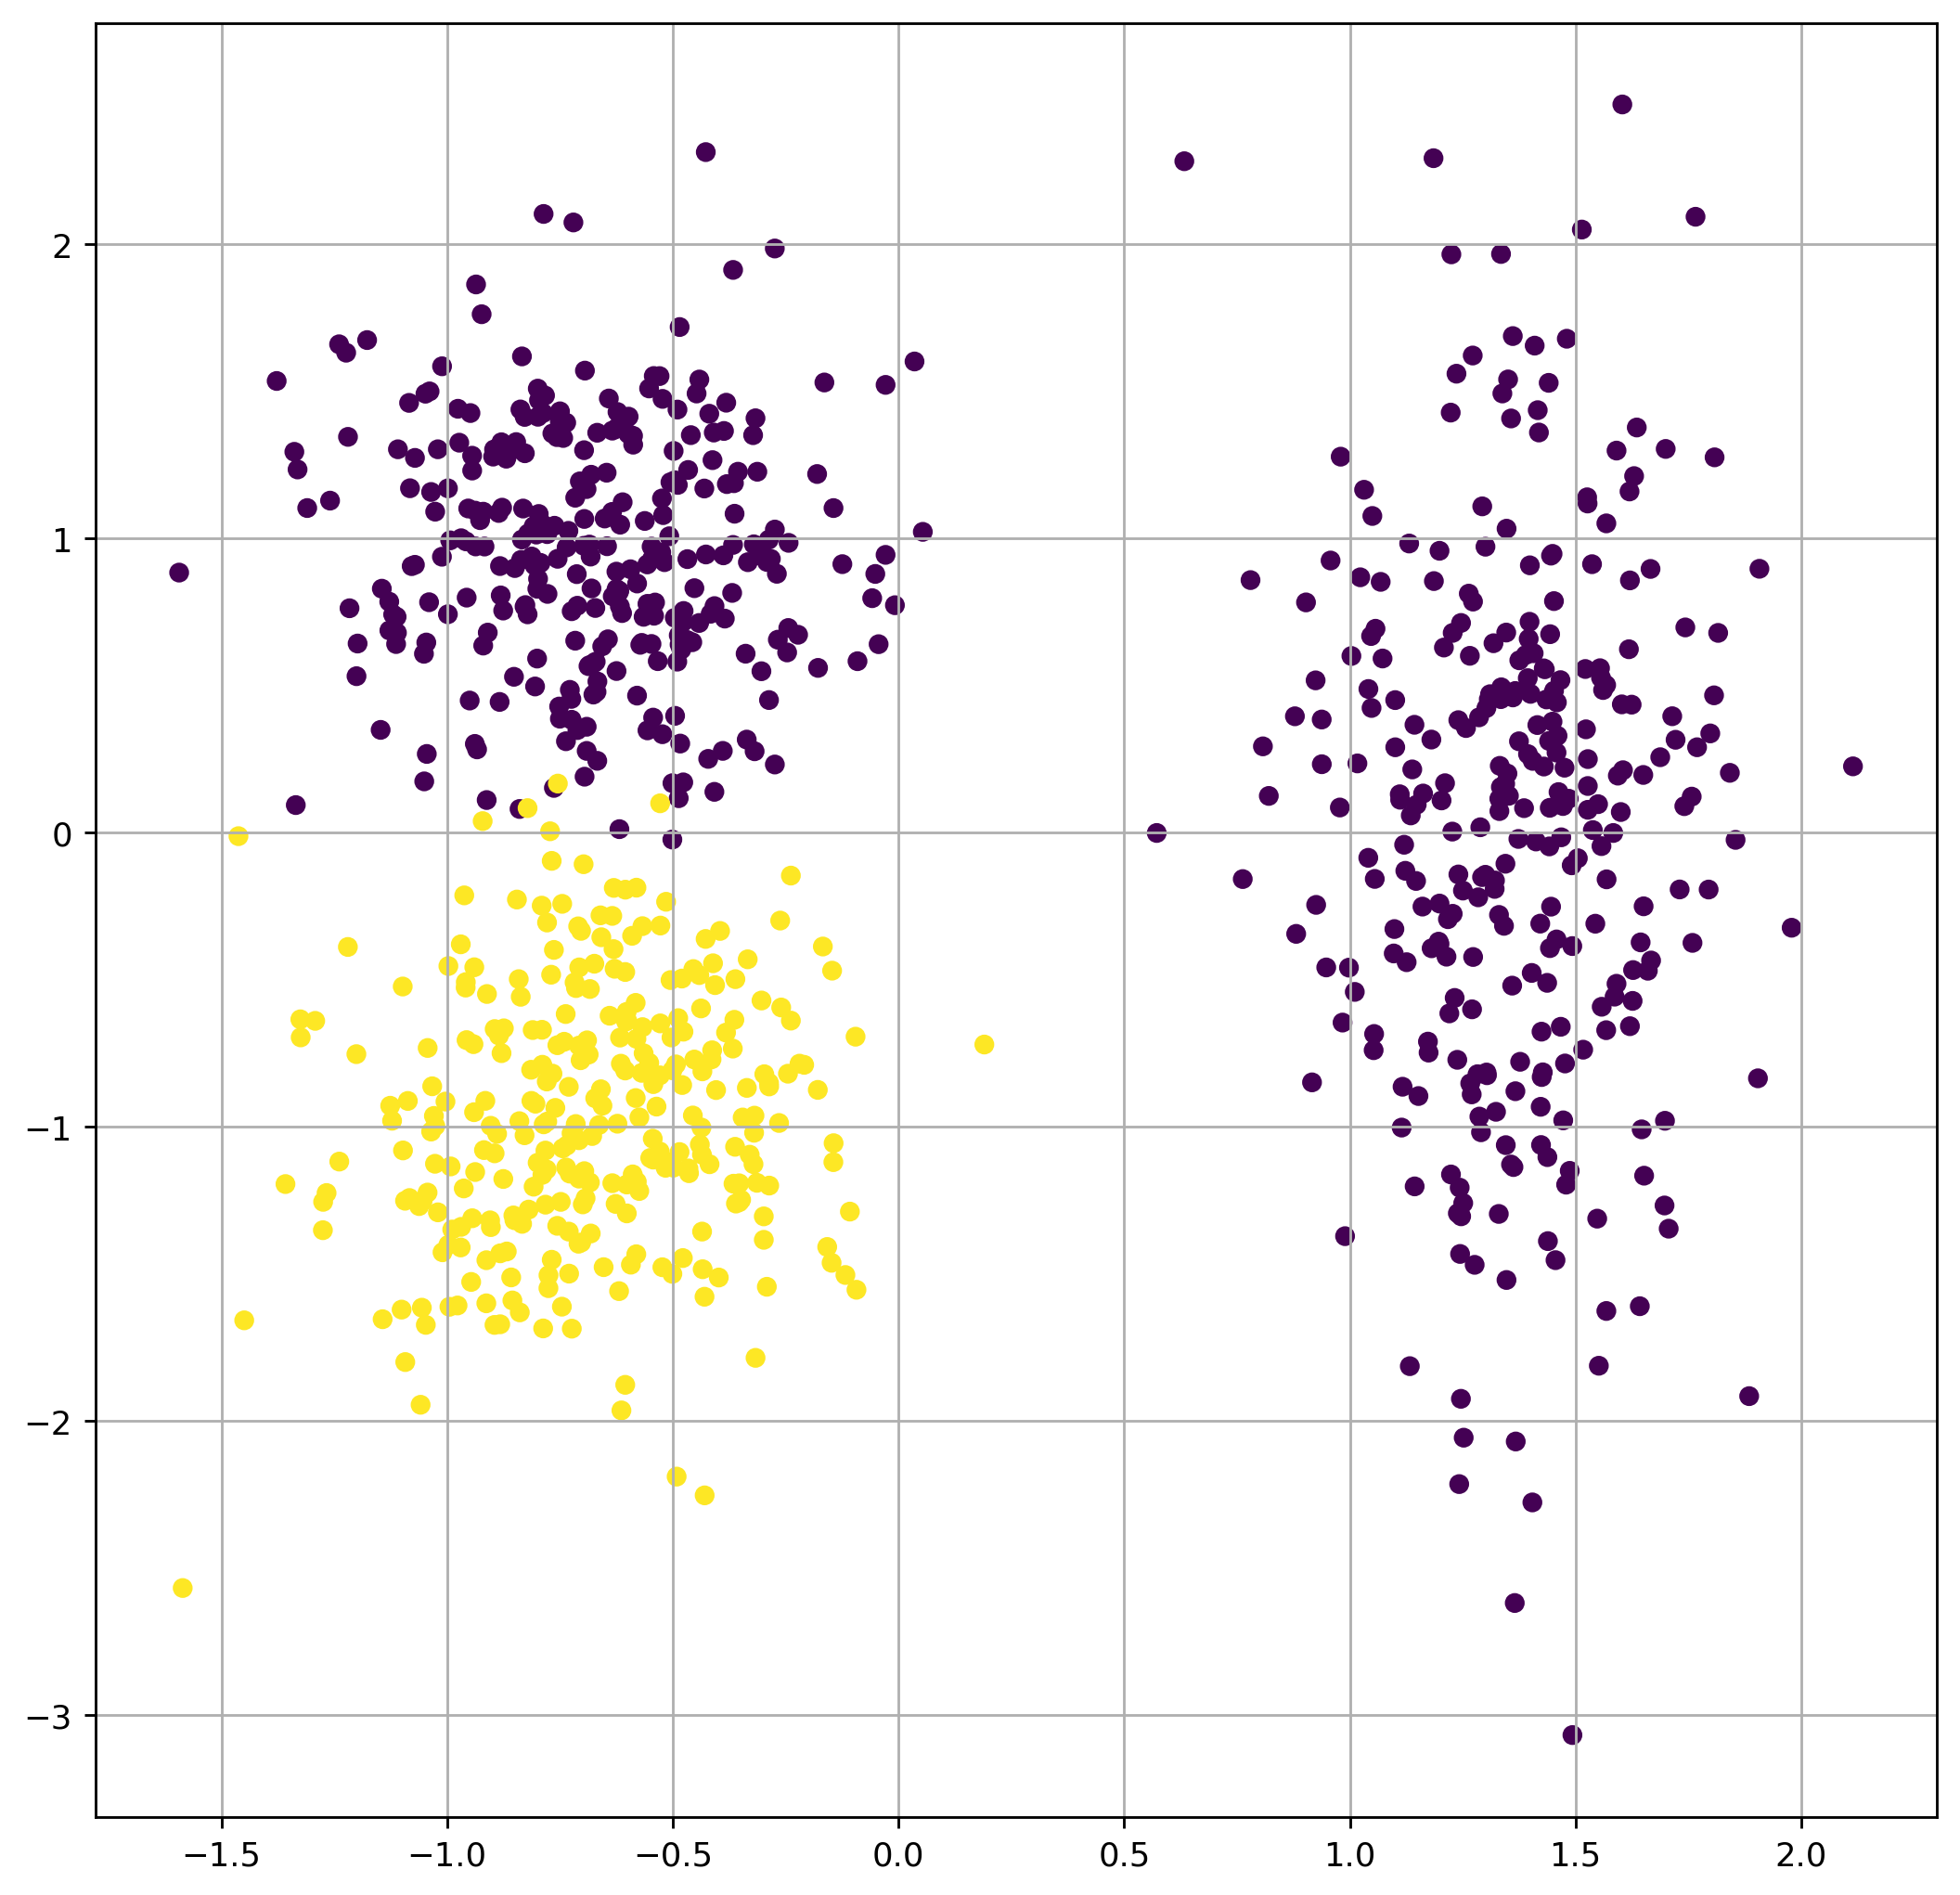
\includegraphics[width=.35\linewidth]{figures/example_groups/groups_centered}}
  ~
  \subfloat[\label{fig:ex-groups-after}]{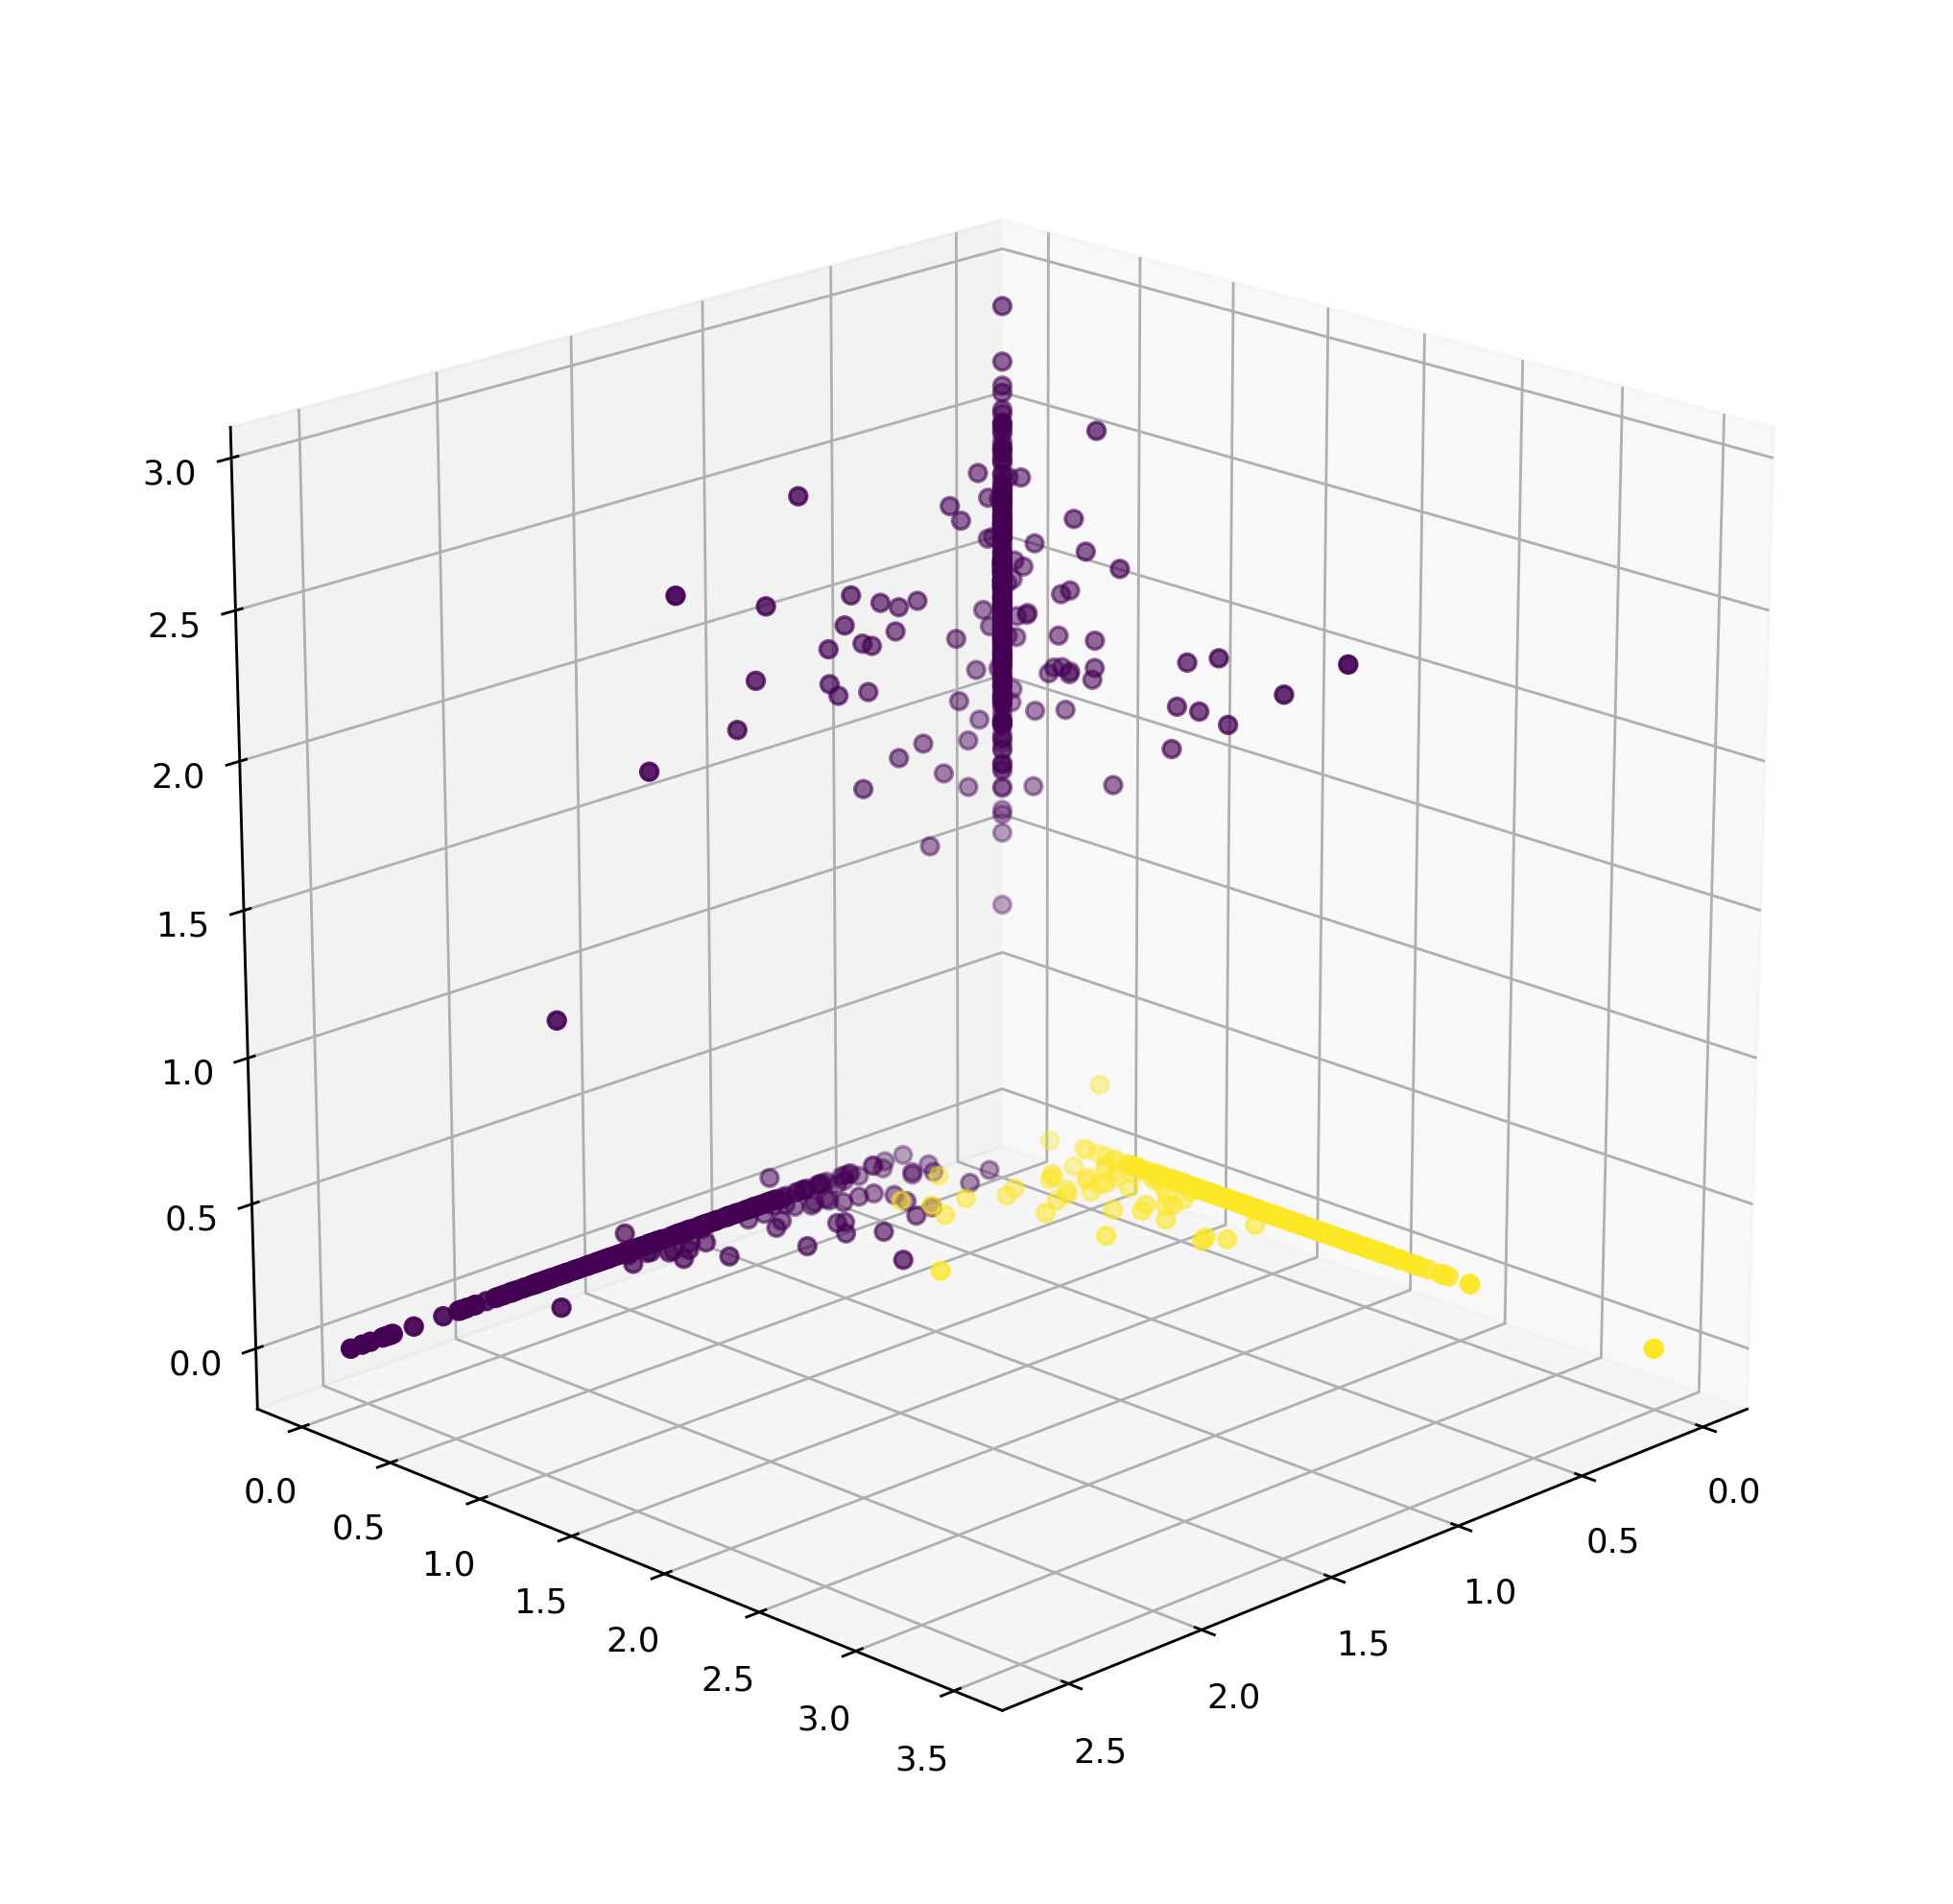
\includegraphics[width=.45\linewidth]{figures/example_groups/groups3d_centered}
  }
  \caption{(a) A 2D feature space with color-coded samples from two classes distributed in three groups. (b) After marker-based batch normalization and convolution with filters obtained from each group, the classes can be more easily detected by two filters in a new 3D feature space.}
  \label{fig:filter}
\end{figure}

Each convolutional layer is trained individually, one layer at a time, to find its filter set ${\cal F}$. The number of filters per layer depends on the clustering technique. We use $K$-means, then the user must specify the number $K=|{\cal F}|$ of filters. After the convolution operation, we apply the ReLU function to eliminate negative activations and the max-pooling operation to aggregate local information. Note that, apart from the initial marker selection, the training process is automatic. We have preserved the convolutional layers' output dimensions and the marker pixels used to find the filters of layer $L+1$ from the output of layer $L$ are always the same for all convolutional layers. Figure~\ref{fig:tree} shows one example of a simple network projected by FLIM for the experiments of the next section. 

\begin{figure}
  \begin{center}
  \tikzset{
    treenode/.style = {shape=rectangle, rounded corners,
                       draw=black, align=center, line width=width},
    specialedge/.style = {line width=1.5pt}
  }

  \begin{tikzpicture}
    [
      grow                    = down,
      sibling distance        = 5em,
      level distance          = 3em,
      edge from parent/.style = {draw=black, -latex},
      every node/.style       = {treenode},
      sloped
    ]
    \node [treenode, fill=tealDeer] (v0) {MarkerBased BatchNorm}
    child {
        node [treenode, fill=tealDeer] {Conv$(60 \times 7 \times 7)$}
        child {
          node [treenode, fill=tealDeer] {ReLU} 
          child {
            node [treenode, fill=tealDeer] {MaxPool$(3\times3)$}
            child {
              node [treenode, fill=tealDeer] {BatchNorm}
              child {
                node [treenode, fill=navyPurple] {Classifier}
                edge from parent
              }
            }
          } 
        }
      };

  \end{tikzpicture}
  \end{center}
  \caption{Example of a network with a single convolutional layer followed by a classifier, as projected by FLIM and used for the experiments in this work.}
  \label{fig:tree}
\end{figure}

\section{Experiments}

We use a dataset from~\cite{8899005}, which contains aerial images with or without one coconut tree for counting. These images belong to a large imagery from  

selected aerial images from WeRobotics and used the same dataset of regions of interest in these images, as provided by\cite{8899005} . The imagery with a resolution of 8cm was captured by the World Bank's UAVs for Disaster Resilience Program, collaborating with WeRobotics and OpenAerialMap in the Kingdom of Tonga in October 2017. The Humanitarian OpenStreetMap community provided the annotation. The dataset consists of 13587 patches of dimensions $90 \times 90$ of coconut (10268) and non-coconut (3319). The latter class has a large variability. The problem of interest is to classify the images in one of the two classes. We only report experiments with one dataset due to the space limitation.

As in reality, labeling images is a costly and time-consuming process, and then we assume that we only knew the correct labels of a small set of samples (one hundred images for each class, totaling two hundred images). That way, we would have only those two hundred images to train any models that we would use to try to solve the problem.

To reduce the impact of chance on the results, we randomly selected three sets of 200 images for training and three sets of 11387 images for testing. We wanted to represent a scenario where the network designer did not have much effort to annotate all these images. From each of these sets of training images, we selected four images using the 2D space projection of the 200 images using the t-SNE. We tried to select images that were part of more cohesive groups. Thus, these images are more likely to have characteristics that represent their group.

\begin{figure}[!t]
    \centering
    \subfloat[\label{fig:markers1}]{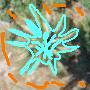
\includegraphics[width=.3\linewidth]{figures/markers1}
    }
    ~
    \subfloat[\label{fig:markers2}]{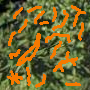
\includegraphics[width=.3\linewidth]{figures/markers2}
    }
    \\
    \subfloat[\label{fig:markers3}]{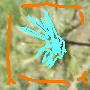
\includegraphics[width=.3\linewidth]{figures/markers3}
    }
    ~
    \subfloat[\label{fig:markers4}]{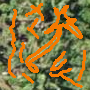
\includegraphics[width=.3\linewidth]{figures/markers4}
    }
    \caption{Markers used for training. (a) Markers on an image which contains a coconut tree. (b) Markers on an image which does not contain a coconut tree. (c) Markers on an image which does not contain a coconut tree. (d) Markers on an image which does not contain a coconut tree.}
    \label{fig:markers}
\end{figure}

We placed markers on these images in regions that we consider important to identify the coconut and non-coconut (more diverse) classes. In Figure \ref{fig:markers} we can the four images of one the splits. With the markers, we created a convolutional layer with filters of dimensions $7 \times 7$ using the method described in Section \ref{sec:method}. The network architecture can be seen in the Figure. We used a classifier similar to that of VGG-16. We used K-means to cluster the coconut tree patches in 30 clusters and the non-coconut tree patches in also 30 clusters to find the convolutional layer filter. 

\begin{table}[!t]
  \begin{center}
  \begin{tabular}{|l|c|c|c|}
  \hline
   Method & Precision & Recall & F-score \\
  \hline\hline
    FLIM + SVM & $0.856 \pm 0.011 $ & $ 0.831 \pm 0.019$ & $ 0.838 \pm 0.017$\\ 
    VGG-FE + SVM & $0.855 \pm 0.001$ & $0.816 \pm 0.007$ & $0.826 \pm 0.006 $ \\\hline
      
    FLIM & $0.863 \pm 0.002$ & $0.849 \pm 0.005$ & $0.854 \pm 0.004$\\
    FLIM-FT & $0.845 \pm 0.003$ & $0.825\pm 0.006$ & $0.832 \pm 0.005$ \\

    VGG & $0.827 \pm 0.003$ & $0.770 \pm 0.016$  & $ 0.784 \pm 0.014$\\
    VGG-FT & $0.872 \pm 0.007$ & $0.844 \pm 0.015$ & $0.851 \pm 0.014 $ \\
   
  \hline
  \end{tabular}
  \end{center}
  \caption{Results.}
  \label{tab:results}
\end{table}


We tested three scenarios: (I) using out method to learn the feature extractor weights and the classifier with backpropagation; (II) using our method as initialization and train the whole model with backpropagation; (III) using SVM Linear as classification. For VGG-16, we tested two scenarios: (IV) initializing with Xavier initialization and training from scratch; (V) using ImageNet weights and training with the training set images. The results can be seen in Table \ref{tab:results}. As the experiments were repeated three times, we reported the mean and standard deviation of each the metrics in the test set. 

\begin{figure}
  \centering
  \subfloat{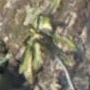
\includegraphics[width=.3\linewidth]{figures/qualitative/ours/upper-coco-108.png}
  }
  ~
  \subfloat{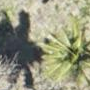
\includegraphics[width=.3\linewidth]{figures/qualitative/ours/upper-coco-2473.png}
  }
  ~
  \subfloat{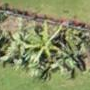
\includegraphics[width=.3\linewidth]{figures/qualitative/ours/upper-non_coco-506.png}
  }
  \\
  \subfloat{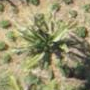
\includegraphics[width=.3\linewidth]{figures/qualitative/vgg/lower-coco-1098.png}
  }
  ~
  \subfloat{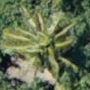
\includegraphics[width=.3\linewidth]{figures/qualitative/vgg/lower-coco-2400.png}
  }
  ~
  \subfloat{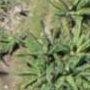
\includegraphics[width=.3\linewidth]{figures/qualitative/vgg/lower-non_coco-105.png}
  }
  \caption{Misclassified images. The first row has images misclassified by the network trained by our method, and the second row has images misclassified by VGG-16. The two first images of a row have coconut trees.}
  \label{fig:ex-classification}
\end{figure}

Our method achieved better precision than conventionally trained VGG, and the difference between precision and recall is much smaller. The Linear SVM did not prove to be a good classifier like the MLP, but, on average, it still got a little better than the VGG-16. Using our method as initialization and training the entire network with backpropagation did not improve the result; this implies that the filters we created are already good filters given the training set. Our feature extractor training method was able to learn good filters from a minimal set of images. VGG has many parameters to learn, so it is susceptible to overfitting with such a small training set. We do not use any technique to handle small data sets to train VGG because we intended to verify our approach viability, and these techniques could also be used with our method. In Figure \ref{fig:ex-classification} we can see examples of misclassified images. In these images, coconut trees appear in different angles, sizes, and shapes, or the boundaries between the coconut tree and the background are tenuous, making it more difficult to identify them. In turn, images that do not contain coconut trees, contain trees that resemble their shape. The network designer could put markers in those images in other to improve the feature extractor.

\begin{figure}
  \centering
  \subfloat[\label{fig:vis-input}]{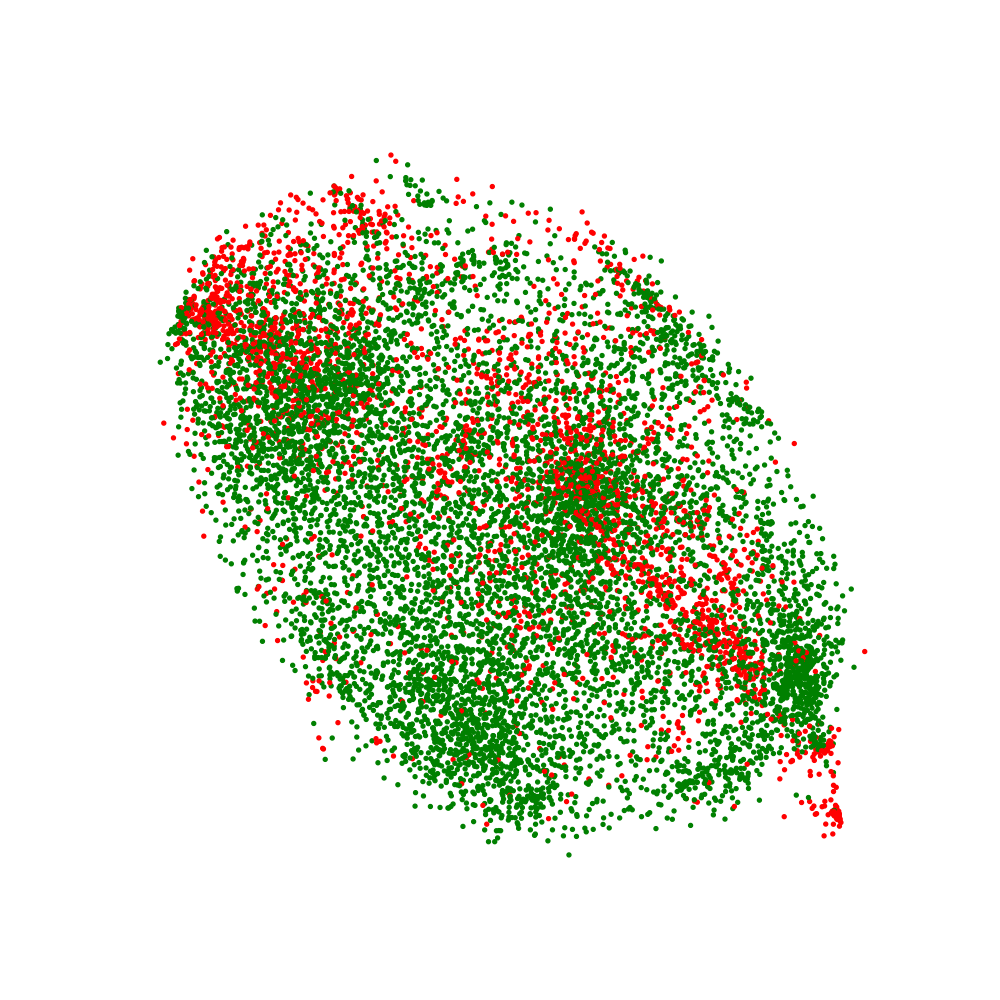
\includegraphics[width=.3\linewidth]{figures/input}
  }
  ~
  \subfloat[\label{fig:vis-feature-extractor}]{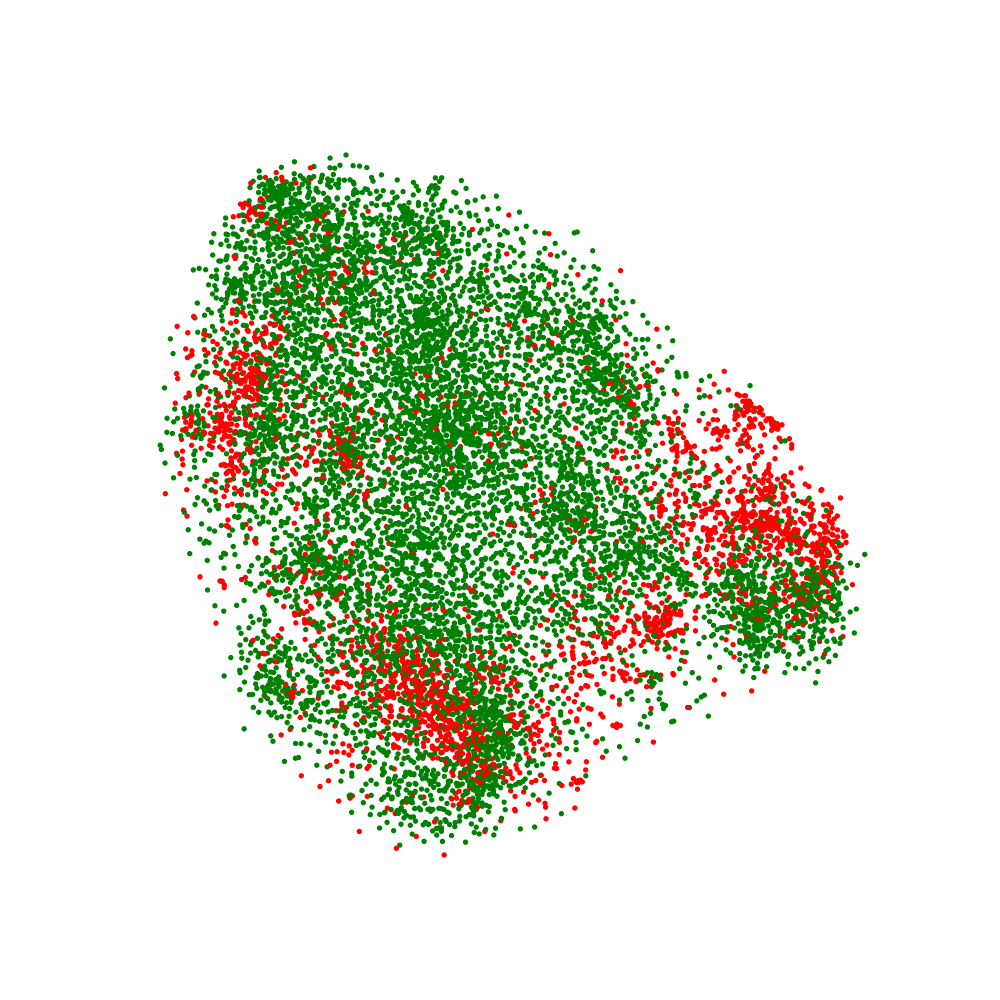
\includegraphics[width=.3\linewidth]{figures/feature_extractor}
  }
  ~
  \subfloat[]{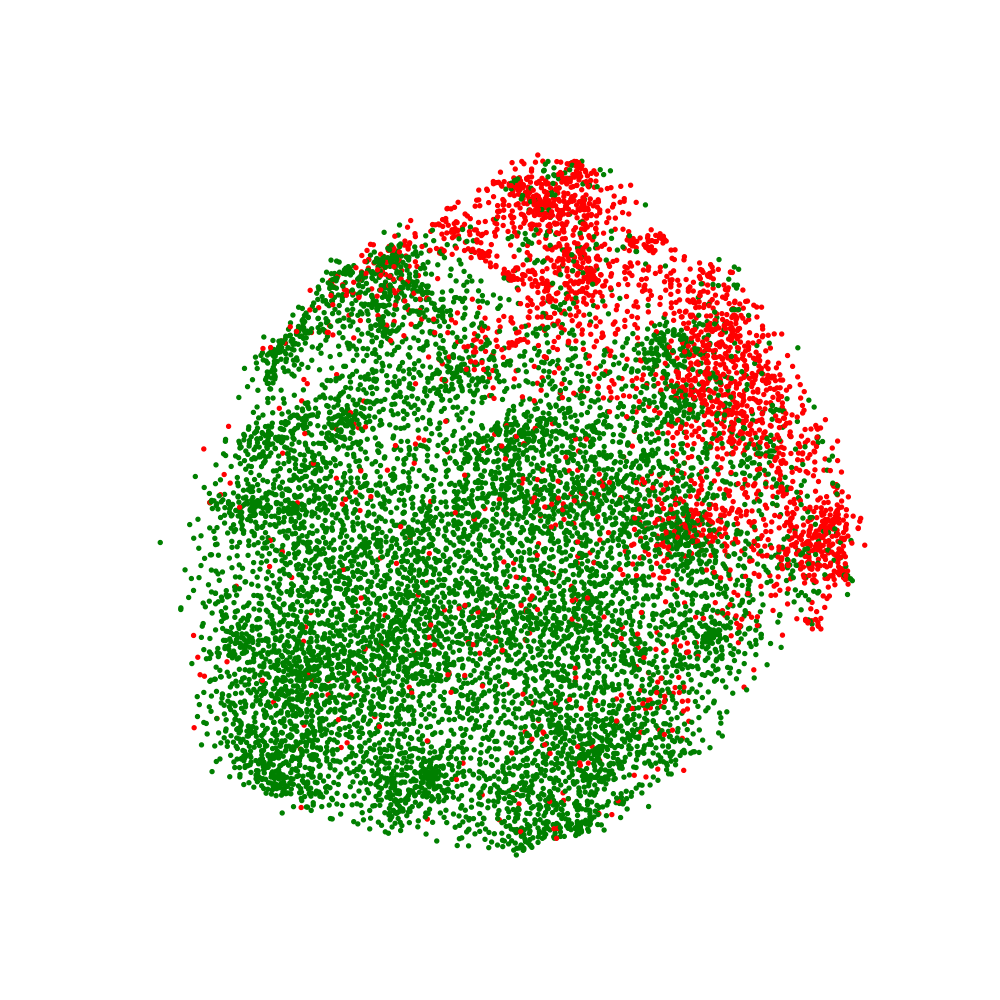
\includegraphics[width=.3\linewidth]{figures/classifier}
  \label{fig:vis-classifier}}
  \caption{This image shows visualizations of the input images and the intermediate layer's outputs. Red points represent background images, and green points represent images that have a coconut tree. The projection from high dimensionality space to 2D was made using t-SNE. The original image shows much overlap between the classes; after applying the feature extractor with only one convolutional layer, we can see that the overlapping decreases considerably. Before the decision layer, the last layer put most of the images from one class on one side and the other on the other side. (a) Visualization of original image feature space. (b) Visualization of the feature extractor's outputs. (c) Visualization of outputs from the last classifier hidden layer.}
\end{figure}

As motivated by Rauber et al. \cite{rauber2016visualizing}, we made projections of three stages of the network using t-SNE \cite{maaten2008visualizing} to understand how the feature extractor trained with our method transforms the image spaces. In Figure \ref{fig:vis-input}, we can see the projection of the original images (in the LAB color space). Red points are images that contain coconut trees, and green points are images that do not contain coconut trees. In the projection in the image of Figure \ref{fig:vis-input}, we see that the images of coconut trees and non-coconut trees are almost entirely overlapping. Coconut tree images are more frequent in some regions but are very dispersed. In the image of Figure \ref{fig:vis-feature-extractor}, we see the projection of the feature extractor output. The coconut tree images are more concentrated, forming some clusters, and it is possible to notice that there is much less overlap. Finally, we see in Figure \ref{fig:vis-classifier} the output of the previous layer of the decision layer of the classifier. The classifier managed to organize conquest and non-coconut images in different regions of space, although there is overlap as the model failed to achieve 100\% accuracy.

\section{Conclusions}

We present a way to train a feature extractor without using backpropagation capable of learning good filters from a minimal set of images. To evaluate the method, we proposed experiments to classify images that contain achievements. Our approach has achieved competitive results with state of the art.

\bibliographystyle{IEEEtran}
\bibliography{bibliography}

\end{document}


